
\large

\chapter*{Simplex Optimization}
\addcontentsline{toc}{chapter}{Simplex Optimization}

\section{Inroduction}
The simplex Nelder-Mead algorithm (Amoeba search) is widely used to
solve unconstrained function minimization problems even the
discontinuous ones or subject to noise. The algorithm is an iterative
process, meaning, it tries to replace the worst solution with a better
one and reorder the simplex nodes. Each iteration, the search area is
moving and deformed based on some rules. To understand the structure of
the algorithm more closely, we begin with introducing some helpful
stuff. Our main goal is :
{\[\min\limits_{\overset{\rightarrow}{X} \in \mathbb{R}^{n}}{f(\overset{\rightarrow}{X})}\]}{\[f:\mathbb{R}^{n}\rightarrow\mathbb{R}\]}Where,
{\(f\)} is the objective function we have discussed earlier and {\(n\)}
is the dimension. And the simplex is a geometric figure that lives in
that {\(n\)} dimension with {\(n + 1\)} vertices. In 2-D, it is a
triangle, so we are going to denote it by {\(\Delta\)} for simplicity
and convenience.
{\[\Delta = ({\overset{\rightarrow}{x}}_{best}\ ,\ {\overset{\rightarrow}{x}}_{other}\ ,\ {\overset{\rightarrow}{x}}_{worst})\]}
\begin{figure}[htbp]
        \centering
        \scalebox{1.1}{


\tikzset{every picture/.style={line width=0.75pt}} %set default line width to 0.75pt        

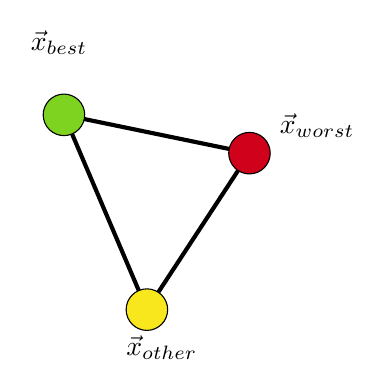
\begin{tikzpicture}[x=0.75pt,y=0.75pt,yscale=-1,xscale=1]
%uncomment if require: \path (0,914); %set diagram left start at 0, and has height of 914

%Straight Lines [id:da0052534278546845226] 
\draw [line width=1.5]    (63.21,89.73) -- (152.59,108.19) ;
%Straight Lines [id:da2220277816214007] 
\draw [line width=1.5]    (103.18,183.58) -- (63.21,89.73) ;
%Straight Lines [id:da006067659711585183] 
\draw [line width=1.5]    (103.18,183.58) -- (152.59,108.19) ;
%Shape: Circle [id:dp15048672252515094] 
\draw  [fill={rgb, 255:red, 126; green, 211; blue, 33 }  ,fill opacity=1 ] (54.01,93.65) .. controls (51.85,88.57) and (54.21,82.7) .. (59.29,80.53) .. controls (64.37,78.37) and (70.25,80.73) .. (72.41,85.81) .. controls (74.57,90.9) and (72.21,96.77) .. (67.13,98.93) .. controls (62.05,101.1) and (56.17,98.73) .. (54.01,93.65) -- cycle ;
%Shape: Circle [id:dp2153424878727488] 
\draw  [fill={rgb, 255:red, 208; green, 2; blue, 27 }  ,fill opacity=1 ] (143.39,112.1) .. controls (141.22,107.02) and (143.59,101.15) .. (148.67,98.99) .. controls (153.75,96.82) and (159.62,99.19) .. (161.79,104.27) .. controls (163.95,109.35) and (161.59,115.22) .. (156.51,117.39) .. controls (151.43,119.55) and (145.55,117.19) .. (143.39,112.1) -- cycle ;
%Shape: Circle [id:dp6498543047529874] 
\draw  [fill={rgb, 255:red, 248; green, 231; blue, 28 }  ,fill opacity=1 ] (93.98,187.49) .. controls (91.82,182.41) and (94.18,176.54) .. (99.26,174.38) .. controls (104.34,172.21) and (110.22,174.58) .. (112.38,179.66) .. controls (114.54,184.74) and (112.18,190.61) .. (107.1,192.78) .. controls (102.02,194.94) and (96.14,192.58) .. (93.98,187.49) -- cycle ;

% Text Node
\draw (46,48) node [anchor=north west][inner sep=0.75pt]   [align=left] {$\displaystyle \vec{x}_{best}$};
% Text Node
\draw (166,88) node [anchor=north west][inner sep=0.75pt]   [align=left] {$\displaystyle \vec{x}_{worst}$};
% Text Node
\draw (92,195) node [anchor=north west][inner sep=0.75pt]   [align=left] {$\displaystyle \vec{x}_{other}$};


\end{tikzpicture}}
        \caption{Initial state of particle at point of time $t$ }
        \label{fig:label}
    \end{figure}

where,

\begin{itemize}
\item
  {\({\overset{\rightarrow}{x}}_{best}\)} is the best solution within
  the vertices
\item
  {\({\overset{\rightarrow}{x}}_{worst}\)} is the worst solution within
  the vertices
\item
  {\({\overset{\rightarrow}{x}}_{other}\)} is the solution in between\\
  That is based on the fact that :\\
  {\[f({\overset{\rightarrow}{x}}_{best}) \leq \ \ f({\overset{\rightarrow}{x}}_{other})\  \leq \ f({\overset{\rightarrow}{x}}_{worst})\]}The
  goal now is to adjust the parameter values of the worst point so that
  the simplex moves towards the minimum of the function with the
  direction of moving determined by the centroid.
\end{itemize}

\section{Mathematical Model of Simplex method}
\subsubsection{Compute Centroid}

The centroid represents the geometric mean between two points. It is
calculated for every pair of vertices in the simplex except for the
worst point.\\
{\[\overline{x} = \frac{1}{n}\sum\limits_{i = 1}^{n}x_{i}\]}In our case
{\(n = 2\)}, the centroid is calculated for
{\({\overset{\rightarrow}{x}}_{best}\)} and
{\({\overset{\rightarrow}{x}}_{other}\)} only through the following
simple equation:\\
{\[\overline{x} = ({\overset{\rightarrow}{x}}_{best} + {\overset{\rightarrow}{x}}_{other})/2\]}Now,
all the operation we are going to execute on the simplex will take place
with respect to the direction of vector
({\(\overline{x} - {\overset{\rightarrow}{x}}_{worst}\)}), second
sub-figure.

\begin{figure}[htp]
\begin{subfigure}{0.5\textwidth}
    \centering
   \scalebox{1.1}{


\tikzset{every picture/.style={line width=0.75pt}} %set default line width to 0.75pt        

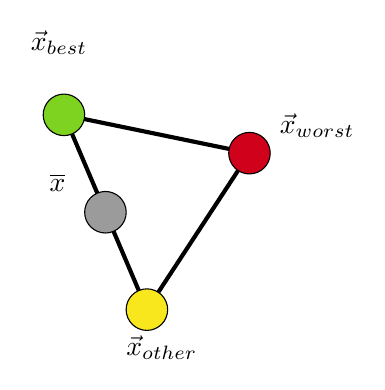
\begin{tikzpicture}[x=0.75pt,y=0.75pt,yscale=-1,xscale=1]
%uncomment if require: \path (0,914); %set diagram left start at 0, and has height of 914

%Straight Lines [id:da8438979087196363] 
\draw [line width=1.5]    (277.21,85.73) -- (366.59,104.19) ;
%Straight Lines [id:da20469279023180365] 
\draw [line width=1.5]    (317.18,179.58) -- (277.21,85.73) ;
%Straight Lines [id:da8334212569541255] 
\draw [line width=1.5]    (317.18,179.58) -- (366.59,104.19) ;
%Shape: Circle [id:dp35373016991770023] 
\draw  [fill={rgb, 255:red, 126; green, 211; blue, 33 }  ,fill opacity=1 ] (268.01,89.65) .. controls (265.85,84.57) and (268.21,78.7) .. (273.29,76.53) .. controls (278.37,74.37) and (284.25,76.73) .. (286.41,81.81) .. controls (288.57,86.9) and (286.21,92.77) .. (281.13,94.93) .. controls (276.05,97.1) and (270.17,94.73) .. (268.01,89.65) -- cycle ;
%Shape: Circle [id:dp40627430744057724] 
\draw  [fill={rgb, 255:red, 208; green, 2; blue, 27 }  ,fill opacity=1 ] (357.39,108.1) .. controls (355.22,103.02) and (357.59,97.15) .. (362.67,94.99) .. controls (367.75,92.82) and (373.62,95.19) .. (375.79,100.27) .. controls (377.95,105.35) and (375.59,111.22) .. (370.51,113.39) .. controls (365.43,115.55) and (359.55,113.19) .. (357.39,108.1) -- cycle ;
%Shape: Circle [id:dp7608960793687913] 
\draw  [fill={rgb, 255:red, 248; green, 231; blue, 28 }  ,fill opacity=1 ] (307.98,183.49) .. controls (305.82,178.41) and (308.18,172.54) .. (313.26,170.38) .. controls (318.34,168.21) and (324.22,170.58) .. (326.38,175.66) .. controls (328.54,180.74) and (326.18,186.61) .. (321.1,188.78) .. controls (316.02,190.94) and (310.14,188.58) .. (307.98,183.49) -- cycle ;
%Shape: Circle [id:dp5171429606236433] 
\draw  [fill={rgb, 255:red, 155; green, 155; blue, 155 }  ,fill opacity=1 ] (287.99,136.57) .. controls (285.83,131.49) and (288.2,125.62) .. (293.28,123.45) .. controls (298.36,121.29) and (304.23,123.65) .. (306.4,128.74) .. controls (308.56,133.82) and (306.19,139.69) .. (301.11,141.85) .. controls (296.03,144.02) and (290.16,141.65) .. (287.99,136.57) -- cycle ;

% Text Node
\draw (260,44) node [anchor=north west][inner sep=0.75pt]   [align=left] {$\displaystyle \vec{x}_{best}$};
% Text Node
\draw (380,84) node [anchor=north west][inner sep=0.75pt]   [align=left] {$\displaystyle \vec{x}_{worst}$};
% Text Node
\draw (306,191) node [anchor=north west][inner sep=0.75pt]   [align=left] {$\displaystyle \vec{x}_{other}$};
% Text Node
\draw (269,113) node [anchor=north west][inner sep=0.75pt]   [align=left] {$\displaystyle \overline{x}$};


\end{tikzpicture}}
  \caption{Intial state of particles}
  \label{fig:sub1}
\end{subfigure}%
\begin{subfigure}{0.5\textwidth}
 \centering
   \scalebox{1.1}{


\tikzset{every picture/.style={line width=0.75pt}} %set default line width to 0.75pt        

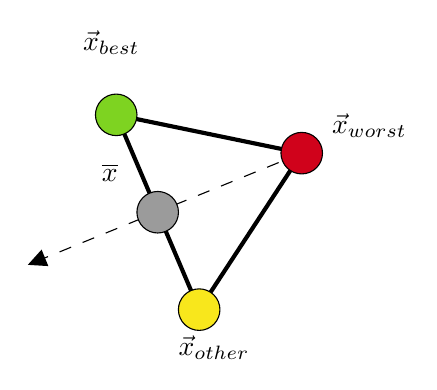
\begin{tikzpicture}[x=0.75pt,y=0.75pt,yscale=-1,xscale=1]
%uncomment if require: \path (0,914); %set diagram left start at 0, and has height of 914

%Straight Lines [id:da3736551905137999] 
\draw [line width=1.5]    (500.21,83.73) -- (589.59,102.19) ;
%Straight Lines [id:da04487834593966644] 
\draw [line width=1.5]    (540.18,177.58) -- (500.21,83.73) ;
%Straight Lines [id:da39512755814535017] 
\draw [line width=1.5]    (540.18,177.58) -- (589.59,102.19) ;
%Shape: Circle [id:dp004075579027117859] 
\draw  [fill={rgb, 255:red, 126; green, 211; blue, 33 }  ,fill opacity=1 ] (491.01,87.65) .. controls (488.85,82.57) and (491.21,76.7) .. (496.29,74.53) .. controls (501.37,72.37) and (507.25,74.73) .. (509.41,79.81) .. controls (511.57,84.9) and (509.21,90.77) .. (504.13,92.93) .. controls (499.05,95.1) and (493.17,92.73) .. (491.01,87.65) -- cycle ;
%Shape: Circle [id:dp6832733573702188] 
\draw  [fill={rgb, 255:red, 248; green, 231; blue, 28 }  ,fill opacity=1 ] (530.98,181.49) .. controls (528.82,176.41) and (531.18,170.54) .. (536.26,168.38) .. controls (541.34,166.21) and (547.22,168.58) .. (549.38,173.66) .. controls (551.54,178.74) and (549.18,184.61) .. (544.1,186.78) .. controls (539.02,188.94) and (533.14,186.58) .. (530.98,181.49) -- cycle ;
%Straight Lines [id:da518882999322084] 
\draw  [dash pattern={on 4.5pt off 4.5pt}]  (589.59,102.19) -- (460.39,154.87) ;
\draw [shift={(457.61,156)}, rotate = 337.82] [fill={rgb, 255:red, 0; green, 0; blue, 0 }  ][line width=0.08]  [draw opacity=0] (8.93,-4.29) -- (0,0) -- (8.93,4.29) -- cycle    ;
%Shape: Circle [id:dp1573898137156733] 
\draw  [fill={rgb, 255:red, 155; green, 155; blue, 155 }  ,fill opacity=1 ] (510.99,134.57) .. controls (508.83,129.49) and (511.2,123.62) .. (516.28,121.45) .. controls (521.36,119.29) and (527.23,121.65) .. (529.4,126.74) .. controls (531.56,131.82) and (529.19,137.69) .. (524.11,139.85) .. controls (519.03,142.02) and (513.16,139.65) .. (510.99,134.57) -- cycle ;
%Shape: Circle [id:dp9607152425984504] 
\draw  [fill={rgb, 255:red, 208; green, 2; blue, 27 }  ,fill opacity=1 ] (580.39,106.1) .. controls (578.22,101.02) and (580.59,95.15) .. (585.67,92.99) .. controls (590.75,90.82) and (596.62,93.19) .. (598.79,98.27) .. controls (600.95,103.35) and (598.59,109.22) .. (593.51,111.39) .. controls (588.43,113.55) and (582.55,111.19) .. (580.39,106.1) -- cycle ;

% Text Node
\draw (483,42) node [anchor=north west][inner sep=0.75pt]   [align=left] {$\displaystyle \vec{x}_{best}$};
% Text Node
\draw (603,82) node [anchor=north west][inner sep=0.75pt]   [align=left] {$\displaystyle \vec{x}_{worst}$};
% Text Node
\draw (529,189) node [anchor=north west][inner sep=0.75pt]   [align=left] {$\displaystyle \vec{x}_{other}$};
% Text Node
\draw (492,106) node [anchor=north west][inner sep=0.75pt]   [align=left] {$\displaystyle \overline{x}$};


\end{tikzpicture}}
  \caption{Final state of particles}
  \label{fig:sub2}
\end{subfigure}
\caption{PSO Animation}
\label{fig:test}
\end{figure}
\subsubsection{Reflection}

Reflection is the first operation we make on the simplex data structure.
It is an attempt to see whether the value of the function at the
reflected point is less than the worst solution. It can be computed
through the upcoming equation.\\
{\[{\overset{\rightarrow}{x}}_{r} = \overline{x} + \alpha(\overline{x} - {\overset{\rightarrow}{x}}_{worst})\]}where
{\(\alpha\)} is the reflection coefficient, positive real-valued
parameter , typically {\(\alpha = 1\)}.

    \begin{figure}[htbp]
        \centering
        \scalebox{1.1}{


\tikzset{every picture/.style={line width=0.75pt}} %set default line width to 0.75pt        

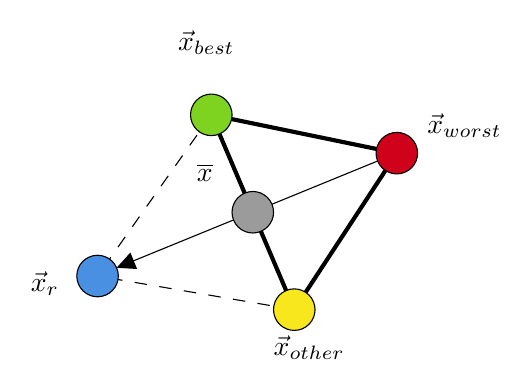
\begin{tikzpicture}[x=0.75pt,y=0.75pt,yscale=-1,xscale=1]
%uncomment if require: \path (0,914); %set diagram left start at 0, and has height of 914

%Straight Lines [id:da39121424549824235] 
\draw [line width=1.5]    (122.21,293.73) -- (211.59,312.19) ;
%Straight Lines [id:da618739710662245] 
\draw [line width=1.5]    (162.18,387.58) -- (122.21,293.73) ;
%Straight Lines [id:da7599011924098371] 
\draw [line width=1.5]    (162.18,387.58) -- (211.59,312.19) ;
%Straight Lines [id:da920148193557524] 
\draw    (211.59,312.19) -- (79.35,366.27) ;
\draw [shift={(76.58,367.41)}, rotate = 337.75] [fill={rgb, 255:red, 0; green, 0; blue, 0 }  ][line width=0.08]  [draw opacity=0] (8.93,-4.29) -- (0,0) -- (8.93,4.29) -- cycle    ;
%Shape: Circle [id:dp8356416145204131] 
\draw  [fill={rgb, 255:red, 155; green, 155; blue, 155 }  ,fill opacity=1 ] (132.99,344.57) .. controls (130.83,339.49) and (133.2,333.62) .. (138.28,331.45) .. controls (143.36,329.29) and (149.23,331.65) .. (151.4,336.74) .. controls (153.56,341.82) and (151.19,347.69) .. (146.11,349.85) .. controls (141.03,352.02) and (135.16,349.65) .. (132.99,344.57) -- cycle ;
%Shape: Circle [id:dp45226827899303657] 
\draw  [fill={rgb, 255:red, 208; green, 2; blue, 27 }  ,fill opacity=1 ] (202.39,316.1) .. controls (200.22,311.02) and (202.59,305.15) .. (207.67,302.99) .. controls (212.75,300.82) and (218.62,303.19) .. (220.79,308.27) .. controls (222.95,313.35) and (220.59,319.22) .. (215.51,321.39) .. controls (210.43,323.55) and (204.55,321.19) .. (202.39,316.1) -- cycle ;
%Straight Lines [id:da7153645519608796] 
\draw  [dash pattern={on 4.5pt off 4.5pt}]  (162.18,387.58) -- (67.4,371.39) ;
%Straight Lines [id:da799114901839753] 
\draw  [dash pattern={on 4.5pt off 4.5pt}]  (122.21,293.73) -- (67.4,371.39) ;
%Shape: Circle [id:dp5444502759814949] 
\draw  [fill={rgb, 255:red, 74; green, 144; blue, 226 }  ,fill opacity=1 ] (76.58,367.41) .. controls (78.77,372.47) and (76.45,378.36) .. (71.38,380.56) .. controls (66.32,382.76) and (60.43,380.43) .. (58.23,375.37) .. controls (56.03,370.3) and (58.36,364.41) .. (63.42,362.21) .. controls (68.49,360.01) and (74.38,362.34) .. (76.58,367.41) -- cycle ;
%Shape: Circle [id:dp26683593943410067] 
\draw  [fill={rgb, 255:red, 126; green, 211; blue, 33 }  ,fill opacity=1 ] (113.01,297.65) .. controls (110.85,292.57) and (113.21,286.7) .. (118.29,284.53) .. controls (123.37,282.37) and (129.25,284.73) .. (131.41,289.81) .. controls (133.57,294.9) and (131.21,300.77) .. (126.13,302.93) .. controls (121.05,305.1) and (115.17,302.73) .. (113.01,297.65) -- cycle ;
%Shape: Circle [id:dp8150487348338344] 
\draw  [fill={rgb, 255:red, 248; green, 231; blue, 28 }  ,fill opacity=1 ] (152.98,391.49) .. controls (150.82,386.41) and (153.18,380.54) .. (158.26,378.38) .. controls (163.34,376.21) and (169.22,378.58) .. (171.38,383.66) .. controls (173.54,388.74) and (171.18,394.61) .. (166.1,396.78) .. controls (161.02,398.94) and (155.14,396.58) .. (152.98,391.49) -- cycle ;

% Text Node
\draw (105,252) node [anchor=north west][inner sep=0.75pt]   [align=left] {$\displaystyle \vec{x}_{best}$};
% Text Node
\draw (225,292) node [anchor=north west][inner sep=0.75pt]   [align=left] {$\displaystyle \vec{x}_{worst}$};
% Text Node
\draw (151,399) node [anchor=north west][inner sep=0.75pt]   [align=left] {$\displaystyle \vec{x}_{other}$};
% Text Node
\draw (114,316) node [anchor=north west][inner sep=0.75pt]   [align=left] {$\displaystyle \overline{x}$};
% Text Node
\draw (34,368) node [anchor=north west][inner sep=0.75pt]   [align=left] {$\displaystyle \vec{x}_{r}$};


\end{tikzpicture}}
        \caption{Initial state of particle at point of time $t$ }
        \label{fig:label}
    \end{figure}


If the objective function at the reflected point is less than the other
point, but not the best, we set the reflected point to the worst.\\
{\[f({\overset{\rightarrow}{x}}_{best}) \leq \ \ f({\overset{\rightarrow}{x}}_{r})\  < \ f({\overset{\rightarrow}{x}}_{other})\quad\;\Longrightarrow\;{\overset{\rightarrow}{x}}_{worst} = {\overset{\rightarrow}{x}}_{r}\]}And
we reorder the vertices as we mentioned above; in fact, we have to
reorder the vertices of the simplex after each operation, which is the
whole point of the algorithm.

\subsubsection{Expansion}

If it happened and the reflected point is better than the best point (in
terms of fitness)
{\(f({\overset{\rightarrow}{x}}_{r}) < \ \ f({\overset{\rightarrow}{x}}_{best})\)}
, maybe we can find better point a bit further from the reflected point,
that is the idea of expansion.\\
{\[{\overset{\rightarrow}{x}}_{e} = {\overset{\rightarrow}{x}}_{r} + \beta({\overset{\rightarrow}{x}}_{r} - \overline{x})\]}where
{\(\beta\)} is the expansion coefficient, with {\(\beta > 1\)} ,
typically {\(\beta = 2\)}.

    \begin{figure}[htbp]
        \centering
        \scalebox{1.1}{


\tikzset{every picture/.style={line width=0.75pt}} %set default line width to 0.75pt        

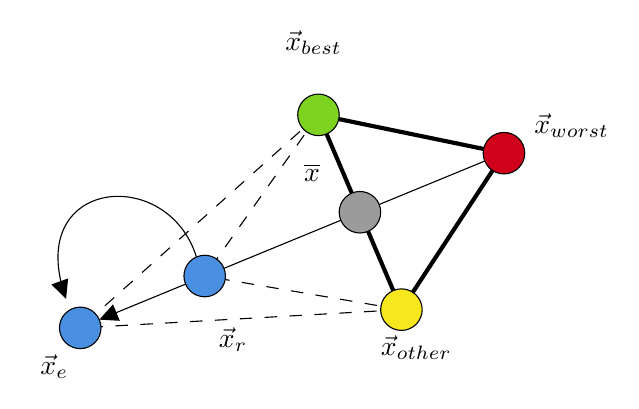
\begin{tikzpicture}[x=0.75pt,y=0.75pt,yscale=-1,xscale=1]
%uncomment if require: \path (0,914); %set diagram left start at 0, and has height of 914

%Straight Lines [id:da11343228301624042] 
\draw [line width=1.5]    (431.21,289.73) -- (520.59,308.19) ;
%Straight Lines [id:da5343513078972191] 
\draw [line width=1.5]    (471.18,383.58) -- (431.21,289.73) ;
%Straight Lines [id:da35681996429433105] 
\draw [line width=1.5]    (471.18,383.58) -- (520.59,308.19) ;
%Straight Lines [id:da35098952534036765] 
\draw    (520.59,308.19) -- (328.38,387.25) ;
\draw [shift={(325.61,388.39)}, rotate = 337.64] [fill={rgb, 255:red, 0; green, 0; blue, 0 }  ][line width=0.08]  [draw opacity=0] (8.93,-4.29) -- (0,0) -- (8.93,4.29) -- cycle    ;
%Shape: Circle [id:dp9759552457158815] 
\draw  [fill={rgb, 255:red, 155; green, 155; blue, 155 }  ,fill opacity=1 ] (441.99,340.57) .. controls (439.83,335.49) and (442.2,329.62) .. (447.28,327.45) .. controls (452.36,325.29) and (458.23,327.65) .. (460.4,332.74) .. controls (462.56,337.82) and (460.19,343.69) .. (455.11,345.85) .. controls (450.03,348.02) and (444.16,345.65) .. (441.99,340.57) -- cycle ;
%Shape: Circle [id:dp25947223717017986] 
\draw  [fill={rgb, 255:red, 208; green, 2; blue, 27 }  ,fill opacity=1 ] (511.39,312.1) .. controls (509.22,307.02) and (511.59,301.15) .. (516.67,298.99) .. controls (521.75,296.82) and (527.62,299.19) .. (529.79,304.27) .. controls (531.95,309.35) and (529.59,315.22) .. (524.51,317.39) .. controls (519.43,319.55) and (513.55,317.19) .. (511.39,312.1) -- cycle ;
%Straight Lines [id:da5926907267680663] 
\draw  [dash pattern={on 4.5pt off 4.5pt}]  (471.18,383.58) -- (376.4,367.39) ;
%Straight Lines [id:da13882970361087188] 
\draw  [dash pattern={on 4.5pt off 4.5pt}]  (431.21,289.73) -- (376.4,367.39) ;
%Shape: Circle [id:dp08877809464082187] 
\draw  [fill={rgb, 255:red, 74; green, 144; blue, 226 }  ,fill opacity=1 ] (385.58,363.41) .. controls (387.77,368.47) and (385.45,374.36) .. (380.38,376.56) .. controls (375.32,378.76) and (369.43,376.43) .. (367.23,371.37) .. controls (365.03,366.3) and (367.36,360.41) .. (372.42,358.21) .. controls (377.49,356.01) and (383.38,358.34) .. (385.58,363.41) -- cycle ;
%Straight Lines [id:da6283525001318553] 
\draw  [dash pattern={on 4.5pt off 4.5pt}]  (471.18,383.58) -- (316.43,392.37) ;
%Straight Lines [id:da46426000871766093] 
\draw  [dash pattern={on 4.5pt off 4.5pt}]  (431.21,289.73) -- (316.43,392.37) ;
%Shape: Circle [id:dp39491065736136166] 
\draw  [fill={rgb, 255:red, 74; green, 144; blue, 226 }  ,fill opacity=1 ] (325.61,388.39) .. controls (327.81,393.46) and (325.48,399.35) .. (320.41,401.54) .. controls (315.35,403.74) and (309.46,401.42) .. (307.26,396.35) .. controls (305.06,391.28) and (307.39,385.39) .. (312.46,383.2) .. controls (317.52,381) and (323.41,383.32) .. (325.61,388.39) -- cycle ;
%Shape: Circle [id:dp8580698815752372] 
\draw  [fill={rgb, 255:red, 248; green, 231; blue, 28 }  ,fill opacity=1 ] (461.98,387.49) .. controls (459.82,382.41) and (462.18,376.54) .. (467.26,374.38) .. controls (472.34,372.21) and (478.22,374.58) .. (480.38,379.66) .. controls (482.54,384.74) and (480.18,390.61) .. (475.1,392.78) .. controls (470.02,394.94) and (464.14,392.58) .. (461.98,387.49) -- cycle ;
%Shape: Circle [id:dp07260801254247773] 
\draw  [fill={rgb, 255:red, 126; green, 211; blue, 33 }  ,fill opacity=1 ] (422.01,293.65) .. controls (419.85,288.57) and (422.21,282.7) .. (427.29,280.53) .. controls (432.37,278.37) and (438.25,280.73) .. (440.41,285.81) .. controls (442.57,290.9) and (440.21,296.77) .. (435.13,298.93) .. controls (430.05,301.1) and (424.17,298.73) .. (422.01,293.65) -- cycle ;
%Curve Lines [id:da945800091817379] 
\draw    (308.46,374.97) .. controls (291.38,320.13) and (358.7,314.11) .. (372.42,358.21) ;
\draw [shift={(309.61,378.39)}, rotate = 250.1] [fill={rgb, 255:red, 0; green, 0; blue, 0 }  ][line width=0.08]  [draw opacity=0] (8.93,-4.29) -- (0,0) -- (8.93,4.29) -- cycle    ;

% Text Node
\draw (414,248) node [anchor=north west][inner sep=0.75pt]   [align=left] {$\displaystyle \vec{x}_{best}$};
% Text Node
\draw (534,288) node [anchor=north west][inner sep=0.75pt]   [align=left] {$\displaystyle \vec{x}_{worst}$};
% Text Node
\draw (460,395) node [anchor=north west][inner sep=0.75pt]   [align=left] {$\displaystyle \vec{x}_{other}$};
% Text Node
\draw (423,312) node [anchor=north west][inner sep=0.75pt]   [align=left] {$\displaystyle \overline{x}$};
% Text Node
\draw (382,391) node [anchor=north west][inner sep=0.75pt]   [align=left] {$\displaystyle \vec{x}_{r}$};
% Text Node
\draw (296,404) node [anchor=north west][inner sep=0.75pt]   [align=left] {$\displaystyle \vec{x}_{e}$};


\end{tikzpicture}}
        \caption{Initial state of particle at point of time $t$ }
        \label{fig:label}
    \end{figure}


Again, we check the quality of the new point
{\({\overset{\rightarrow}{x}}_{e}\)} , if it is better than the
reflected point, then we are in the right direction, if not we assign
the reflected point to the worst point normally which means, we have
done a bad attempt .\\
{\[f({\overset{\rightarrow}{x}}_{e}) < \ \ f({\overset{\rightarrow}{x}}_{r})\quad\;\Longrightarrow\;{\overset{\rightarrow}{x}}_{worst} = {\overset{\rightarrow}{x}}_{e}\]}{\[f({\overset{\rightarrow}{x}}_{e}) \geq \ \ f({\overset{\rightarrow}{x}}_{r})\quad\;\Longrightarrow\;{\overset{\rightarrow}{x}}_{worst} = {\overset{\rightarrow}{x}}_{r}\]}


\subsubsection{Contraction}

If the reflected is worse from the beginning, then we can minimize the
damage by contracting the simplex whether inside or outside, whichever
is better.


\paragraph{Inside contraction}

when the reflected point is worse than all including the worst point, we
try to contract the simplex towards the worst point, perhaps we get a
better solution.\\
{\[f({\overset{\rightarrow}{x}}_{r}) \geq \ \ f({\overset{\rightarrow}{x}}_{worst})\]}{\[{\overset{\rightarrow}{x}}_{c} = \overline{x} + \gamma({\overset{\rightarrow}{x}}_{worst} - \overline{x})\]}where
{\(\gamma\)} is the contraction coefficient, with {\(0 < \gamma < 1\)} ,
typically {\(\gamma = \frac{1}{2}\)}.\\
if the fitness value is better at the contracted point than the worst
point, we replace the worst point with the contracted one, if not we
moved in the wrong direction, maybe we have to go backwards.\\
{\[f({\overset{\rightarrow}{x}}_{c}) < \ \ f({\overset{\rightarrow}{x}}_{worst})\quad\;\Longrightarrow\;{\overset{\rightarrow}{x}}_{worst} = {\overset{\rightarrow}{x}}_{c}\]}

    \begin{figure}[htbp]
        \centering
        \scalebox{1.1}{


\tikzset{every picture/.style={line width=0.75pt}} %set default line width to 0.75pt        

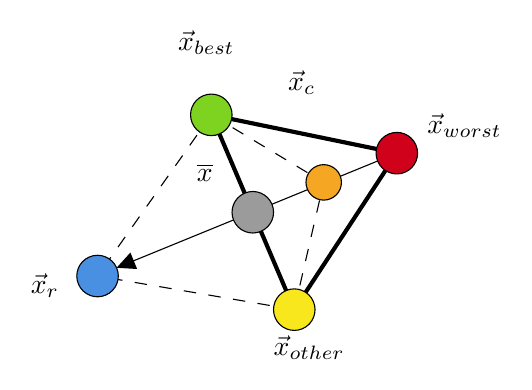
\begin{tikzpicture}[x=0.75pt,y=0.75pt,yscale=-1,xscale=1]
%uncomment if require: \path (0,914); %set diagram left start at 0, and has height of 914

%Straight Lines [id:da4445133148332976] 
\draw [line width=1.5]    (129.21,515.73) -- (218.59,534.19) ;
%Straight Lines [id:da8072652131616453] 
\draw [line width=1.5]    (169.18,609.58) -- (129.21,515.73) ;
%Straight Lines [id:da26520550089423445] 
\draw [line width=1.5]    (169.18,609.58) -- (218.59,534.19) ;
%Straight Lines [id:da04667789058155303] 
\draw    (218.59,534.19) -- (86.35,588.27) ;
\draw [shift={(83.58,589.41)}, rotate = 337.75] [fill={rgb, 255:red, 0; green, 0; blue, 0 }  ][line width=0.08]  [draw opacity=0] (8.93,-4.29) -- (0,0) -- (8.93,4.29) -- cycle    ;
%Shape: Circle [id:dp13626854632058039] 
\draw  [fill={rgb, 255:red, 155; green, 155; blue, 155 }  ,fill opacity=1 ] (139.99,566.57) .. controls (137.83,561.49) and (140.2,555.62) .. (145.28,553.45) .. controls (150.36,551.29) and (156.23,553.65) .. (158.4,558.74) .. controls (160.56,563.82) and (158.19,569.69) .. (153.11,571.85) .. controls (148.03,574.02) and (142.16,571.65) .. (139.99,566.57) -- cycle ;
%Shape: Circle [id:dp1389172126099203] 
\draw  [fill={rgb, 255:red, 208; green, 2; blue, 27 }  ,fill opacity=1 ] (209.39,538.1) .. controls (207.22,533.02) and (209.59,527.15) .. (214.67,524.99) .. controls (219.75,522.82) and (225.62,525.19) .. (227.79,530.27) .. controls (229.95,535.35) and (227.59,541.22) .. (222.51,543.39) .. controls (217.43,545.55) and (211.55,543.19) .. (209.39,538.1) -- cycle ;
%Straight Lines [id:da9263850358947512] 
\draw  [dash pattern={on 4.5pt off 4.5pt}]  (169.18,609.58) -- (74.4,593.39) ;
%Straight Lines [id:da334078503397518] 
\draw  [dash pattern={on 4.5pt off 4.5pt}]  (129.21,515.73) -- (74.4,593.39) ;
%Shape: Circle [id:dp17305345317593535] 
\draw  [fill={rgb, 255:red, 74; green, 144; blue, 226 }  ,fill opacity=1 ] (83.58,589.41) .. controls (85.77,594.47) and (83.45,600.36) .. (78.38,602.56) .. controls (73.32,604.76) and (67.43,602.43) .. (65.23,597.37) .. controls (63.03,592.3) and (65.36,586.41) .. (70.42,584.21) .. controls (75.49,582.01) and (81.38,584.34) .. (83.58,589.41) -- cycle ;
%Straight Lines [id:da5749691409395861] 
\draw  [dash pattern={on 4.5pt off 4.5pt}]  (169.18,609.58) -- (183.36,548.27) ;
%Straight Lines [id:da9253197524181758] 
\draw  [dash pattern={on 4.5pt off 4.5pt}]  (129.21,515.73) -- (183.36,548.27) ;
%Shape: Circle [id:dp59696029177814] 
\draw  [fill={rgb, 255:red, 126; green, 211; blue, 33 }  ,fill opacity=1 ] (120.01,519.65) .. controls (117.85,514.57) and (120.21,508.7) .. (125.29,506.53) .. controls (130.37,504.37) and (136.25,506.73) .. (138.41,511.81) .. controls (140.57,516.9) and (138.21,522.77) .. (133.13,524.93) .. controls (128.05,527.1) and (122.17,524.73) .. (120.01,519.65) -- cycle ;
%Shape: Circle [id:dp8536947286133791] 
\draw  [fill={rgb, 255:red, 248; green, 231; blue, 28 }  ,fill opacity=1 ] (159.98,613.49) .. controls (157.82,608.41) and (160.18,602.54) .. (165.26,600.38) .. controls (170.34,598.21) and (176.22,600.58) .. (178.38,605.66) .. controls (180.54,610.74) and (178.18,616.61) .. (173.1,618.78) .. controls (168.02,620.94) and (162.14,618.58) .. (159.98,613.49) -- cycle ;
%Shape: Circle [id:dp9385455494879282] 
\draw  [fill={rgb, 255:red, 245; green, 166; blue, 35 }  ,fill opacity=1 ] (175.51,551.61) .. controls (173.66,547.28) and (175.68,542.26) .. (180.02,540.41) .. controls (184.35,538.56) and (189.37,540.58) .. (191.22,544.92) .. controls (193.06,549.26) and (191.05,554.28) .. (186.71,556.12) .. controls (182.37,557.97) and (177.35,555.95) .. (175.51,551.61) -- cycle ;

% Text Node
\draw (112,474) node [anchor=north west][inner sep=0.75pt]   [align=left] {$\displaystyle \vec{x}_{best}$};
% Text Node
\draw (232,514) node [anchor=north west][inner sep=0.75pt]   [align=left] {$\displaystyle \vec{x}_{worst}$};
% Text Node
\draw (158,621) node [anchor=north west][inner sep=0.75pt]   [align=left] {$\displaystyle \vec{x}_{other}$};
% Text Node
\draw (121,538) node [anchor=north west][inner sep=0.75pt]   [align=left] {$\displaystyle \overline{x}$};
% Text Node
\draw (41,591) node [anchor=north west][inner sep=0.75pt]   [align=left] {$\displaystyle \vec{x}_{r}$};
% Text Node
\draw (165,493) node [anchor=north west][inner sep=0.75pt]   [align=left] {$\displaystyle \vec{x}_{c}$};


\end{tikzpicture}}
        \caption{Initial state of particle at point of time $t$ }
        \label{fig:label}
    \end{figure}



\paragraph{Outside contraction}

When the reflected point is, however, worse than the ``other'' point ,
but better than the worst, we can contract in the outside direction
(towards the reflected point).\\
{\[f({\overset{\rightarrow}{x}}_{other}) \leq \ \ f({\overset{\rightarrow}{x}}_{r})\  < \ f({\overset{\rightarrow}{x}}_{worst})\]}{\[{\overset{\rightarrow}{x}}_{c} = \overline{x} + \gamma({\overset{\rightarrow}{x}}_{r} - \overline{x})\]}And
we also check weather we are going to accept the new point or not.\\
{\[f({\overset{\rightarrow}{x}}_{c}) < \ \ f({\overset{\rightarrow}{x}}_{r})\quad\;\Longrightarrow\;{\overset{\rightarrow}{x}}_{worst} = {\overset{\rightarrow}{x}}_{c}\]}

    \begin{figure}[htbp]
        \centering
        \scalebox{1.1}{


\tikzset{every picture/.style={line width=0.75pt}} %set default line width to 0.75pt        

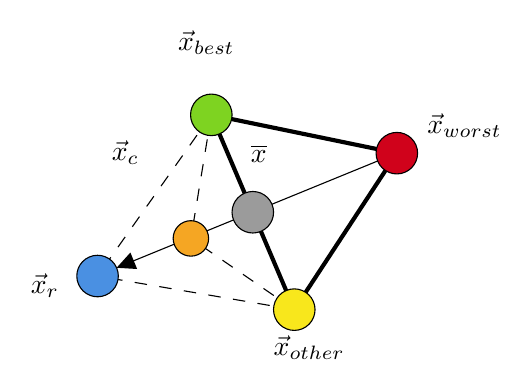
\begin{tikzpicture}[x=0.75pt,y=0.75pt,yscale=-1,xscale=1]
%uncomment if require: \path (0,914); %set diagram left start at 0, and has height of 914

%Straight Lines [id:da20472677135319306] 
\draw [line width=1.5]    (432.21,511.73) -- (521.59,530.19) ;
%Straight Lines [id:da15196510915112627] 
\draw [line width=1.5]    (472.18,605.58) -- (432.21,511.73) ;
%Straight Lines [id:da8014030305919331] 
\draw [line width=1.5]    (472.18,605.58) -- (521.59,530.19) ;
%Straight Lines [id:da3522320622069264] 
\draw    (521.59,530.19) -- (389.35,584.27) ;
\draw [shift={(386.58,585.41)}, rotate = 337.75] [fill={rgb, 255:red, 0; green, 0; blue, 0 }  ][line width=0.08]  [draw opacity=0] (8.93,-4.29) -- (0,0) -- (8.93,4.29) -- cycle    ;
%Shape: Circle [id:dp036939575554771675] 
\draw  [fill={rgb, 255:red, 155; green, 155; blue, 155 }  ,fill opacity=1 ] (442.99,562.57) .. controls (440.83,557.49) and (443.2,551.62) .. (448.28,549.45) .. controls (453.36,547.29) and (459.23,549.65) .. (461.4,554.74) .. controls (463.56,559.82) and (461.19,565.69) .. (456.11,567.85) .. controls (451.03,570.02) and (445.16,567.65) .. (442.99,562.57) -- cycle ;
%Shape: Circle [id:dp010246195714737727] 
\draw  [fill={rgb, 255:red, 208; green, 2; blue, 27 }  ,fill opacity=1 ] (512.39,534.1) .. controls (510.22,529.02) and (512.59,523.15) .. (517.67,520.99) .. controls (522.75,518.82) and (528.62,521.19) .. (530.79,526.27) .. controls (532.95,531.35) and (530.59,537.22) .. (525.51,539.39) .. controls (520.43,541.55) and (514.55,539.19) .. (512.39,534.1) -- cycle ;
%Straight Lines [id:da017687923938115357] 
\draw  [dash pattern={on 4.5pt off 4.5pt}]  (472.18,605.58) -- (377.4,589.39) ;
%Straight Lines [id:da40232054931076844] 
\draw  [dash pattern={on 4.5pt off 4.5pt}]  (432.21,511.73) -- (377.4,589.39) ;
%Shape: Circle [id:dp9492518387184166] 
\draw  [fill={rgb, 255:red, 74; green, 144; blue, 226 }  ,fill opacity=1 ] (386.58,585.41) .. controls (388.77,590.47) and (386.45,596.36) .. (381.38,598.56) .. controls (376.32,600.76) and (370.43,598.43) .. (368.23,593.37) .. controls (366.03,588.3) and (368.36,582.41) .. (373.42,580.21) .. controls (378.49,578.01) and (384.38,580.34) .. (386.58,585.41) -- cycle ;
%Straight Lines [id:da36492452425530564] 
\draw  [dash pattern={on 4.5pt off 4.5pt}]  (472.18,605.58) -- (422.36,571.27) ;
%Straight Lines [id:da2809967890037388] 
\draw  [dash pattern={on 4.5pt off 4.5pt}]  (432.21,511.73) -- (422.36,571.27) ;
%Shape: Circle [id:dp6259185945253334] 
\draw  [fill={rgb, 255:red, 126; green, 211; blue, 33 }  ,fill opacity=1 ] (423.01,515.65) .. controls (420.85,510.57) and (423.21,504.7) .. (428.29,502.53) .. controls (433.37,500.37) and (439.25,502.73) .. (441.41,507.81) .. controls (443.57,512.9) and (441.21,518.77) .. (436.13,520.93) .. controls (431.05,523.1) and (425.17,520.73) .. (423.01,515.65) -- cycle ;
%Shape: Circle [id:dp54940765139848] 
\draw  [fill={rgb, 255:red, 248; green, 231; blue, 28 }  ,fill opacity=1 ] (462.98,609.49) .. controls (460.82,604.41) and (463.18,598.54) .. (468.26,596.38) .. controls (473.34,594.21) and (479.22,596.58) .. (481.38,601.66) .. controls (483.54,606.74) and (481.18,612.61) .. (476.1,614.78) .. controls (471.02,616.94) and (465.14,614.58) .. (462.98,609.49) -- cycle ;
%Shape: Circle [id:dp024904628738977364] 
\draw  [fill={rgb, 255:red, 245; green, 166; blue, 35 }  ,fill opacity=1 ] (414.51,574.61) .. controls (412.66,570.28) and (414.68,565.26) .. (419.02,563.41) .. controls (423.35,561.56) and (428.37,563.58) .. (430.22,567.92) .. controls (432.06,572.26) and (430.05,577.28) .. (425.71,579.12) .. controls (421.37,580.97) and (416.35,578.95) .. (414.51,574.61) -- cycle ;

% Text Node
\draw (415,470) node [anchor=north west][inner sep=0.75pt]   [align=left] {$\displaystyle \vec{x}_{best}$};
% Text Node
\draw (535,510) node [anchor=north west][inner sep=0.75pt]   [align=left] {$\displaystyle \vec{x}_{worst}$};
% Text Node
\draw (461,617) node [anchor=north west][inner sep=0.75pt]   [align=left] {$\displaystyle \vec{x}_{other}$};
% Text Node
\draw (450,525) node [anchor=north west][inner sep=0.75pt]   [align=left] {$\displaystyle \overline{x}$};
% Text Node
\draw (344,587) node [anchor=north west][inner sep=0.75pt]   [align=left] {$\displaystyle \vec{x}_{r}$};
% Text Node
\draw (383,523) node [anchor=north west][inner sep=0.75pt]   [align=left] {$\displaystyle \vec{x}_{c}$};


\end{tikzpicture}}
        \caption{Initial state of particle at point of time $t$ }
        \label{fig:label}
    \end{figure}


\paragraph{Shrinking}

The idea of shrinking is to minimize the damage from a failed
contraction, that is when
{\(f(x_{c}) > \min\left\lbrack f(x_{worst}),f(x_{r}) \right\rbrack\)},
This can be done by moving the worst point and the other point towards
the best point by :\\
{\[{\overset{\rightarrow}{x^{\ast}}}_{worst} = {\overset{\rightarrow}{x}}_{best} + \delta({\overset{\rightarrow}{x}}_{worst} - {\overset{\rightarrow}{x}}_{best})\]}{\[{\overset{\rightarrow}{x^{\ast}}}_{other} = {\overset{\rightarrow}{x}}_{best} + \delta({\overset{\rightarrow}{x}}_{other} - {\overset{\rightarrow}{x}}_{best})\]}where
{\(\delta\)} is the contraction coefficient, with {\(0 < \delta < 1\)} ,
traditionally {\(\delta = \frac{1}{2}\)}.

    \begin{figure}[htbp]
        \centering
        \scalebox{1.1}{


\tikzset{every picture/.style={line width=0.75pt}} %set default line width to 0.75pt        

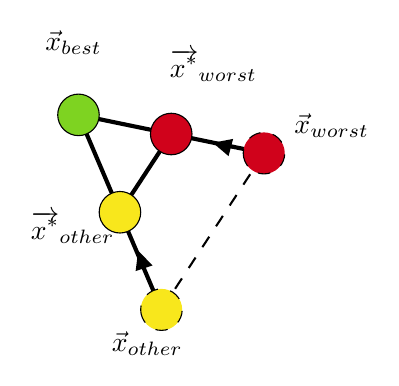
\begin{tikzpicture}[x=0.75pt,y=0.75pt,yscale=-1,xscale=1]
%uncomment if require: \path (0,914); %set diagram left start at 0, and has height of 914

%Straight Lines [id:da8580338020212668] 
\draw [line width=1.5]    (181.9,727.57) -- (157.19,765.26) ;
%Straight Lines [id:da18381718101649303] 
\draw [line width=1.5]    (137.21,718.34) -- (226.59,736.79) ;
%Straight Lines [id:da6854404681605493] 
\draw [line width=1.5]    (177.18,812.18) -- (137.21,718.34) ;
%Straight Lines [id:da10735852785770827] 
\draw [line width=0.75]  [dash pattern={on 4.5pt off 4.5pt}]  (177.18,812.18) -- (226.59,736.79) ;
%Shape: Circle [id:dp9142287215370377] 
\draw  [fill={rgb, 255:red, 126; green, 211; blue, 33 }  ,fill opacity=1 ] (128.01,722.26) .. controls (125.85,717.18) and (128.21,711.31) .. (133.29,709.14) .. controls (138.37,706.98) and (144.25,709.34) .. (146.41,714.42) .. controls (148.57,719.5) and (146.21,725.38) .. (141.13,727.54) .. controls (136.05,729.71) and (130.17,727.34) .. (128.01,722.26) -- cycle ;
%Shape: Circle [id:dp15650187124587034] 
\draw  [fill={rgb, 255:red, 208; green, 2; blue, 27 }  ,fill opacity=1 ][dash pattern={on 4.5pt off 4.5pt}] (217.39,740.71) .. controls (215.22,735.63) and (217.59,729.76) .. (222.67,727.59) .. controls (227.75,725.43) and (233.62,727.79) .. (235.79,732.88) .. controls (237.95,737.96) and (235.59,743.83) .. (230.51,745.99) .. controls (225.43,748.16) and (219.55,745.79) .. (217.39,740.71) -- cycle ;
%Shape: Circle [id:dp10064624056752591] 
\draw  [fill={rgb, 255:red, 248; green, 231; blue, 28 }  ,fill opacity=1 ][dash pattern={on 4.5pt off 4.5pt}] (167.98,816.1) .. controls (165.82,811.02) and (168.18,805.15) .. (173.26,802.98) .. controls (178.34,800.82) and (184.22,803.18) .. (186.38,808.27) .. controls (188.54,813.35) and (186.18,819.22) .. (181.1,821.38) .. controls (176.02,823.55) and (170.14,821.18) .. (167.98,816.1) -- cycle ;
%Shape: Circle [id:dp5873160187999378] 
\draw  [fill={rgb, 255:red, 208; green, 2; blue, 27 }  ,fill opacity=1 ] (172.7,731.49) .. controls (170.54,726.41) and (172.9,720.53) .. (177.98,718.37) .. controls (183.06,716.2) and (188.94,718.57) .. (191.1,723.65) .. controls (193.26,728.73) and (190.9,734.6) .. (185.82,736.77) .. controls (180.74,738.93) and (174.86,736.57) .. (172.7,731.49) -- cycle ;
%Shape: Circle [id:dp20399214913459796] 
\draw  [fill={rgb, 255:red, 248; green, 231; blue, 28 }  ,fill opacity=1 ] (147.99,769.18) .. controls (145.83,764.1) and (148.2,758.23) .. (153.28,756.06) .. controls (158.36,753.9) and (164.23,756.26) .. (166.4,761.34) .. controls (168.56,766.43) and (166.19,772.3) .. (161.11,774.46) .. controls (156.03,776.63) and (150.16,774.26) .. (147.99,769.18) -- cycle ;
%Straight Lines [id:da7948845140831879] 
\draw    (212.61,734.61) -- (204.88,732.56) ;
\draw [shift={(201.98,731.79)}, rotate = 14.83] [fill={rgb, 255:red, 0; green, 0; blue, 0 }  ][line width=0.08]  [draw opacity=0] (8.93,-4.29) -- (0,0) -- (8.93,4.29) -- cycle    ;
%Straight Lines [id:da29396453136809986] 
\draw    (170.61,797.61) -- (166.93,786.64) ;
\draw [shift={(165.98,783.79)}, rotate = 71.48] [fill={rgb, 255:red, 0; green, 0; blue, 0 }  ][line width=0.08]  [draw opacity=0] (8.93,-4.29) -- (0,0) -- (8.93,4.29) -- cycle    ;

% Text Node
\draw (120,676.61) node [anchor=north west][inner sep=0.75pt]   [align=left] {$\displaystyle \vec{x}_{best}$};
% Text Node
\draw (240,716.61) node [anchor=north west][inner sep=0.75pt]   [align=left] {$\displaystyle \vec{x}_{worst}$};
% Text Node
\draw (152,821.61) node [anchor=north west][inner sep=0.75pt]   [align=left] {$\displaystyle \vec{x}_{other}$};
% Text Node
\draw (113,763.61) node [anchor=north west][inner sep=0.75pt]   [align=left] {$\displaystyle \overrightarrow{x^{*}}_{other}$};
% Text Node
\draw (180,685.61) node [anchor=north west][inner sep=0.75pt]   [align=left] {$\displaystyle \overrightarrow{x^{*}}_{worst}$};


\end{tikzpicture}}
        \caption{Initial state of particle at point of time $t$ }
        \label{fig:label}
    \end{figure}


We do all of the previous until we reach the predefined maximum
iterations or we cannot do better by reaching certain threshold, which
can be done by checking the convergence each iteration


\paragraph{Convergence}

We say that , the simplex has converged to the best solution if it is
sufficiently compact meaning that the distance between the each pair of
vertices is adequately small.\\
{\[\sigma = 2\ .\left\lbrack \ \frac{f({\overset{\rightarrow}{x}}_{worst}) - f({\overset{\rightarrow}{x}}_{best})}{f({\overset{\rightarrow}{x}}_{worst}) + f({\overset{\rightarrow}{x}}_{best}) + \epsilon} \right\rbrack\]}where
{\(\epsilon\)} is a tolerance defined based on the nature of the
problem. Each iteration we check if :\\
{\[\sigma < \epsilon\]}if not we proceed until the condition prevails.

